% ---------------------------------------------------------------------------------------------------------------
% TEMPLATE EM LATEX PARA TRABALHO DE CONCLUSÃO DE CURSO DA URI ERECHIM
% (ESTE TEMPLATE NÃO É UM PROJETO OFICIAL DA URI) CONSULTE SEU ORIETADOR CASO QUEIRA UTILIZA-LO
% Este template foi baseado no template da Universidade Tecnológica Federal do Paraná UTFPR
%
% Template baseado no projeto: http://tcc.tsi.gp.utfpr.edu.br/paginas/modelos-latex-da-utfpr
%
%----------------------------------------------------------------------------------------------------------------
% Codificação: UTF-8
% LaTeX:  abnTeX2
% ---------------------------------------------------------------------------------------------------------------


% CARREGA CLASSE PERSONALIZADA COM AS NORMAS DA URI-----------------------------------------------------------
\documentclass[oneside]{template-config/uri-abntex2} %oneside -> impressão apenas frente

% INCLUI ARQUIVOS DE CONFIGURAÇÕES-------------------------------------------------------------------------------
% REFERÊNCIAS------------------------------------------------------------------
\usepackage[%
    alf,
    abnt-emphasize=bf,
    bibjustif,
    recuo=0cm,
    abnt-url-package=url,       % Utiliza o pacote url
    abnt-refinfo=yes,           % Utiliza o estilo bibliográfico abnt-refinfo
    abnt-etal-cite=3,
    abnt-etal-list=3,
    abnt-thesis-year=final
]{abntex2cite}                  % Configura as citações bibliográficas conforme a norma ABNT

% PACOTES----------------------------------------------------------------------
\usepackage[utf8]{inputenc}                                 % Codificação do documento
\usepackage[T1]{fontenc}                                    % Seleção de código de fonte
\usepackage{booktabs}                                       % Réguas horizontais em tabelas
\usepackage{color, colortbl}                                % Controle das cores
\usepackage{float}                                          % Necessário para tabelas/figuras em ambiente multi-colunas
\usepackage{graphicx}                                       % Inclusão de gráficos e figuras
\usepackage{icomma}                                         % Uso de vírgulas em expressões matemáticas
\usepackage{indentfirst}                                    % Indenta o primeiro parágrafo de cada seção
\usepackage{microtype}                                      % Melhora a justificação do documento
\usepackage{multirow, array}                                % Permite tabelas com múltiplas linhas e colunas
\usepackage{subeqnarray}                                    % Permite subnumeração de equações
\usepackage{lastpage}                                       % Para encontrar última página do documento
\usepackage{verbatim}                                       % Permite apresentar texto tal como escrito no documento, ainda que sejam comandos Latex
\usepackage{amsfonts, amssymb, amsmath}                     % Fontes e símbolos matemáticos
\usepackage[algoruled, portuguese]{algorithm2e}             % Permite escrever algoritmos em português
%\usepackage[scaled]{helvet}                                % Usa a fonte Helvetica
\usepackage{times}                                          % Usa a fonte Times
%\usepackage{palatino}                                      % Usa a fonte Palatino
%\usepackage{lmodern}                                       % Usa a fonte Latin Modern
\usepackage[bottom]{footmisc}                               % Mantém as notas de rodapé sempre na mesma posição
\usepackage{ae, aecompl}                                    % Fontes de alta qualidade
\usepackage{latexsym}                                       % Símbolos matemáticos
\usepackage{lscape}                                         % Permite páginas em modo "paisagem"
%\usepackage{picinpar}                                      % Dispor imagens em parágrafos
%\usepackage{scalefnt}
\usepackage{setspace}                                       % Permite redimensionar tamanho da fonte
%\usepackage{subfig}                                        % Posicionamento de figuras
%\usepackage{upgreek}                                       % Fonte letras gregas

% Retira Hifenização de todo o template (opcional) não está errado utilizar isso
\usepackage{hyphenat}
\tolerance=1
\emergencystretch=\maxdimen
\hyphenpenalty=10000
\hbadness=10000
\hyphenchar\font=-1
\sloppy                                     

% Redefine a fonte para uma fonte similar a Arial (fonte Helvetica)
% \renewcommand*\familydefault{\sfdefault}
% Configura todo o documento para times new roman
\renewcommand{\familydefault}{ptm}

% CONFIGURAÇÕES DE APARÊNCIA DO PDF FINAL--------------------------------------
\makeatletter
\hypersetup{%
    portuguese,
    colorlinks=true,   % true: "links" coloridos; false: "links" em caixas de texto
    linkcolor=black,    % Define cor dos "links" internos
    citecolor=black,    % Define cor dos "links" para as referências bibliográficas
    filecolor=black,    % Define cor dos "links" para arquivos
    urlcolor=black,     % Define a cor dos "hiperlinks"
    breaklinks=true,
    pdftitle={\@title},
    pdfauthor={\@author},
    pdfkeywords={abnt, latex, abntex, abntex2}
}
\makeatother

% ALTERA O ASPECTO DA COR AZUL--------------------------------------------------
\definecolor{blue}{RGB}{41,5,195}

% REDEFINIÇÃO DE LABELS---------------------------------------------------------
\renewcommand{\algorithmautorefname}{Algoritmo}
\def\equationautorefname~#1\null{Equa\c c\~ao~(#1)\null}

% CRIA ÍNDICE REMISSIVO---------------------------------------------------------
\makeindex

% HIFENIZAÇÃO DE PALAVRAS QUE NÃO ESTÃO NO DICIONÁRIO---------------------------
\hyphenation{%
    qua-dros-cha-ve
    Kat-sa-gge-los
}



% INCLUI ARQUIVOS DO TRABALHO DE CONCLUSÃO DE CURSO (PRÉ-TEXTUAIS, TEXTUAIS, PÓS-TEXTUAIS)-----------------------

% INSERE CAPA E FOLHA DE ROSTO
% CAPA---------------------------------------------------------------------------------------------------

% ORIENTAÇÕES GERAIS-------------------------------------------------------------------------------------
% Caso algum dos campos não se aplique ao seu trabalho, como por exemplo,
% se não houve coorientador, apenas deixe vazio.
% Exemplos: 
% \coorientador{}
% \departamento{}

% DADOS DO TRABALHO--------------------------------------------------------------------------------------
\titulo{Pesquisa e Implementação de uma Aplicação Paralela Utilizando o Paradigma de Grafos de Dependências de Tarefas}
%Análise de desempenho de uma aplicação paralela utilizando o paralelismo de tarefas direcionado a um ambiente de execução heterogêneo
\titleabstract{Research and Implementation of a Parallel Application Using the Task Dependency Graph Paradigm}
\autor{Marcos Vinicius de Moura Lima}
\autorcitacao{LIMA, Marcos Vinicius} % Sobrenome em maiúsculo
\local{ERECHIM - RS}
\data{2018}

% NATUREZA DO TRABALHO-----------------------------------------------------------------------------------
% Opções: 
% - Projeto de Conclusão de Curso (Disciplina de Projeto)
% - Trabalho de Conclusão de Curso (se for Graduação)
% - Dissertação (se for Mestrado)
% - Tese (se for Doutorado)
% - Projeto de Qualificação (se for Mestrado ou Doutorado)
\projeto{Projeto de Conclusão de Curso}

% TÍTULO ACADÊMICO---------------------------------------------------------------------------------------
% Opções:
% - Bacharel ou Tecnólogo (Se a natureza for Trabalho de Conclusão de Curso)
% - Mestre (Se a natureza for Dissertação)
% - Doutor (Se a natureza for Tese)
% - Mestre ou Doutor (Se a natureza for Projeto de Qualificação)
\tituloAcademico{Bacharel}

% ÁREA DE CONCENTRAÇÃO E LINHA DE PESQUISA---------------------------------------------------------------
% Se a natureza for Trabalho de Conclusão de Curso, deixe ambos os campos vazios
% Se for programa de Pós-graduação, indique a área de concentração e a linha de pesquisa
\areaconcentracao{}
\linhapesquisa{}

% DADOS DA INSTITUIÇÃO-----------------------------------------------------------------------------------
% Se a natureza for Trabalho de Conclusão de Curso, coloque o nome do curso de graduação em "programa"
% Formato para o logo da Instituição: \logoinstituicao{<escala>}{<caminho/nome do arquivo>}
\instituicao{Universidade Regional Integrada do Alto Uruguai e das Missões - Campus de Erechim}
\departamento{Departamento de Engenharias e Ciência da Computação}
\programa{Curso de Ciência da Computação}
\disciplina{Projeto de Conclusão de Curso}
%\logoinstituicao{0.2}{dados/figuras/logo-instituicao.png} 

% DADOS DOS ORIENTADORES---------------------------------------------------------------------------------
% No caso do Projeto de Conclusão vai o nome do professor que ministra a disciplina
\orientador{Fábio A. Zanin}
%\orientador[Orientadora:]{Nome da orientadora}
\instOrientador{Instituição do orientador}

\coorientador{Nome do coorientador}
%\coorientador[Coorientadora:]{Nome da coorientadora}
\instCoorientador{Instituição do coorientador}

% FOLHA DE ROSTO--------------------------------------------------------------------------------------------------------

% Os dados podem ser alterados em /text-elements/pre-textuais/capa.tex

% PROJETO DE CONCLUSÂO DE CURSO
% \preambulo{{\imprimirprojeto} elaborado e apresentado na disciplina de {\imprimirdisciplina}, Curso de {\imprimirprograma}, {\imprimirdepartamento} da {\imprimirinstituicao}.}

% TRABALHO DE CONCLUSÃO DE CURSO
\preambulo{{\imprimirprojeto} apresentado como requisito parcial à obtenção do grau de {\imprimirtituloAcademico}, {\imprimirdepartamento} da {\imprimirinstituicao}.}

% DISSERTAÇÃO DE MESTRADO
% \preambulo{{\imprimirprojeto} apresentada ao Programa de \mbox{Pós-graduação} da {\imprimirinstituicao}, como requisito parcial para obtenção do título de {\imprimirtituloAcademico}.}

% TESE DE DOUTORADO
% \preambulo{{\imprimirprojeto} apresentada ao Programa de \mbox{Pós-graduação} da {\imprimirinstituicao}, como requisito parcial para a obtenção do título de {\imprimirtituloAcademico}.}

% PROJETO DE QUALIFICAÇÃO DE MESTRADO OU DOUTORADO
%\preambulo{{\imprimirprojeto} apresentado ao Programa de \mbox{Pós-graduação} da {\imprimirinstituicao}, como requisito parcial para a obtenção do título de {\imprimirtituloAcademico}.}

% OBSERVAÇÕES-----------------------------------------------------------------------------------------------------------
% Altere este arquivo APENAS comentando as linhas que não se aplicam ao tipo de trabalho acadêmico desejado.

% \include{text-elements/pre-textuais/folha-aprovação}

\begin{document}

\pretextual
\imprimircapa                                               	           % Comando para imprimir Capa
\imprimirfolhaderosto{}                                     		   % Comando para imprimir Folha de rosto
% \imprimirfolhadeaprovacao
% INSERE ELEMENTOS PRÉ-TEXTUAIS
% % DEDICATÓRIA------------------------------------------------------------------

\renewcommand{\dedicatorianame}{DEDICATÓRIA}

\begin{dedicatoria}

Altere este texto inserindo a dedicatória do seu trabalho. 

\end{dedicatoria}
          			   % Dedicatória
% % AGRADECIMENTOS---------------------------------------------------------------

\begin{agradecimentos}[AGRADECIMENTOS]

Edite e coloque aqui os agradecimentos às pessoas e/ou instituições que contribuíram para a realização do trabalho.

É obrigatório o agradecimento às instituições de fomento à pesquisa que financiaram total ou parcialmente o trabalho, inclusive no que diz respeito à concessão de bolsas.

\end{agradecimentos}
        			   % Agradecimentos
% % EPÍGRAFE---------------------------------------------------------------------

\renewcommand{\epigraphname}{EPÍGRAFE}

\begin{epigrafe}

\textit{Eu denomino meu campo de Gestão do Conhecimento, mas você não pode gerenciar conhecimento. Ninguém pode. O que pode fazer - o que a empresa pode fazer - é gerenciar o ambiente que otimize o conhecimento.}
\\  \hspace*{\fill} (PRUSAK, Laurence, 1997)

\end{epigrafe}

% OBSERVAÇÕES------------------------------------------------------------------
% Altere o texto para inserir a epígrafe do seu trabalho
              			   % Epígrafe
% RESUMO--------------------------------------------------------------------------------

\begin{resumo}[RESUMO]
\begin{SingleSpacing}

% % Não altere esta seção do texto--------------------------------------------------------
% \imprimirautorcitacao. \imprimirtitulo. \imprimirdata. \pageref {LastPage} f. \imprimirprojeto\ – \imprimirprograma, \imprimirinstituicao. \imprimirlocal, \imprimirdata.\\
% %---------------------------------------------------------------------------------------

O desenvolvimento de aplicações paralelas voltadas a arquiteturas heterogêneas pode vir a ser algo desafiador, pois, nessas arquiteturas, os componentes são formados por processadores \emph{multi-core} (CPUs) e placas gráficas (GPUs).
O programador, então, deverá distribuir as instruções que devem ser executadas em alguns destes componentes, embusca de alcançar o melhor desempenho da aplicação.
Existem atualmente ambientes que se encarregam desta distribuição das instruções para os componentes da arquitetura como, por exemplo, o StarPU. 
Tendo em vista isto, este trabalho explorará o paradigma de Paralelismo de Tarefas, aplicando-o em uma simulação de Transferência de Calor em uma placa metálica bidimensional e executada no ambiente StarPU.
Ao final deste trabalho, serão coletados dados sobre esta aplicação buscando avaliar seu desempenho neste ambiente, comparando com a versão sequencial da aplicação.\\

\textbf{Palavras-chave}: Aplicação Paralela. Arquiteturas Heterogêneas. Computação de Alto Desempenho.

\end{SingleSpacing}
\end{resumo}             			   % Resumo em Português
% ABSTRACT--------------------------------------------------------------------------------

\begin{resumo}[ABSTRACT]
\begin{SingleSpacing}

% % Não altere esta seção do texto--------------------------------------------------------
% \imprimirautorcitacao. \imprimirtitleabstract. \imprimirdata. \pageref {LastPage} f. \imprimirprojeto\ – \imprimirprograma, \imprimirinstituicao. \imprimirlocal, \imprimirdata.\\
% %---------------------------------------------------------------------------------------

Elemento obrigatório em tese, dissertação, monografia e TCC. É a versão do resumo em português para o idioma de divulgação internacional. Deve ser antecedido pela referência do estudo. Deve aparecer em folha distinta do resumo em língua portuguesa e seguido das palavras representativas do conteúdo do estudo, isto é, das palavras-chave. Sugere-se a elaboração do resumo (Abstract) e das palavras-chave (Keywords) em inglês; para resumos em outras línguas, que não o inglês, consultar o departamento / curso de origem.\\

\textbf{Keywords}: Word. Second Word. Another word.

\end{SingleSpacing}
\end{resumo}

% OBSERVAÇÕES---------------------------------------------------------------------------
% Altere o texto inserindo o Abstract do seu trabalho.
% Escolha de 3 a 5 palavras ou termos que descrevam bem o seu trabalho
             		           % Resumo em Inglês
% % Lista de Figuras----------------------------------------------------------------

\pdfbookmark[0]{\listfigurename}{lof}
\listoffigures*
\cleardoublepage

% OBSERVAÇÕES---------------------------------------------------------------------
% Este arquivo não precisa de ser alterado, pois a lista é gerada automaticamente.
   % Lista de Figuras
% % LISTA DE QUADROS----------------------------------------------------------------

\renewcommand{\listofquadrosname}{LISTA DE QUADROS}

\pdfbookmark[0]{\listofquadrosname}{loq}
\listofquadros*
\cleardoublepage

% OBSERVAÇÕES---------------------------------------------------------------------
% Este arquivo não necessita de ser editado. A lista é gerada automaticamente.
   % Lista de Quadros
% % LISTA DE TABELAS-------------------------------------------------------------

\pdfbookmark[0]{\listtablename}{lot}
\listoftables*
\cleardoublepage

% OBSERVAÇÕES-------------------------------------------------------------------
% Este arquivo não precisa ser alterado, pois a lista é gerada automaticamente.
         		   % Lista de Tabelas
% LISTA DE ABREVIATURAS E SIGLAS----------------------------------------------------------

\begin{siglas}
    \item[ABNT] Associação Brasileira de Normas Técnicas
    \item[DECOM] Departamento de Computação
\end{siglas}

% OBSERVAÇÕES-----------------------------------------------------------------------------
% Altere a lista acima para definir os acrônimos e siglas utilizados neste trabalho
          		   % Lista de Abreviaturas e Siglas
% % LISTA DE SÍMBOLOS------------------------------------------------------------

\begin{simbolos}
    \item[$ \Gamma $] Letra grega Gama
    \item[$ \lambda $] Comprimento de onda
    \item[$ \in $] Pertence
\end{simbolos}

% OBSERVAÇÕES-------------------------------------------------------------------
% Altere a lista acima para definir os símbolos utilizados no trabalho
        		   % Lista de Símbolos
% % LISTA DE ALGORITMOS----------------------------------------------------------

\newcommand{\algoritmoname}{Algoritmo}
\renewcommand{\listalgorithmcfname}{LISTA DE ALGORITMOS}

\floatname{algocf}{\algoritmoname}
\newlistof{listofalgoritmos}{loa}{\listalgoritmoname}
\newlistentry{algocf}{loa}{0}

\counterwithout{algocf}{chapter}
\renewcommand{\cftalgocfname}{\algoritmoname\space}
\renewcommand*{\cftalgocfaftersnum}{\hfill--\hfill}

\pdfbookmark[0]{\listalgorithmcfname}{loa}
\listofalgorithms
\cleardoublepage

% OBSERVAÇÕES------------------------------------------------------------------
% Este arquivo não precisa ser alterado, pois a lista é gerada automaticamente.
   % Lista de Algoritmos
% SUMÁRIO----------------------------------------------------------------------

\renewcommand{\contentsname}{SUMÁRIO}

\pdfbookmark[0]{\contentsname}{toc}
\tableofcontents*
\cleardoublepage

% OBSERVAÇÕES-------------------------------------------------------------------
% Este arquivo não precisa ser alterado, pois o sumário é gerado automaticamente.
               			   % Sumário

\textual
% INSERE ELEMENTOS TEXTUAIS
% INTRODUÇÃO-------------------------------------------------------------------

\chapter{INTRODUÇÃO}
\label{chap:introducao}

Arquiteturas Heterogêneas são compostas pelo uso de diferentes tipos de componentes em um mesmo nó computacional. Geralmente essas arquiteturas são compostas por CPUs - (\emph{Central Processing Unit}) e aceleradores, como por exemplo, a GPU - (\emph{Graphics Processing Unit}). Atualmente, muitos fabricantes de chips estão integrando a CPU junto com aceleradores em um mesmo chip, como por exemplo o \emph{Intel Graphics}. 

Por mais que esse tipo de arquitetura aumente o desempenho e diminua o gasto energético, o desenvolvimento de aplicações paralelas para arquiteturas heterogêneas é de certa forma visto como algo desafiador. Para o desenvolvedor conseguir aproveitar totalmente os componentes e recursos, o mesmo deverá identificar e distribuir as instruções mais adequadas em alguns destes componentes, para então tentar alcançar o melhor desempenho da aplicação. Atualmente existem ambientes que se encarregam desta distribuição das instruções para os componentes da arquitetura, como por exemplo, o \emph{StarPU}.

Neste contexto, o trabalho proposto explorará a programação de aplicações paralelas baseadas em tarefas, utilizando o paradigma de Grafo de Dependência de Tarefas. Nesse paradigma, o código da aplicação registra a criação de tarefas e a dependência de dados que existe entre elas. Esse registro de criação de tarefas é direcionado a um ambiente de execução, que se encarrega de distribuir as tarefas de maneira igualitária entre os recursos computacionais.

Como aplicação, será desenvolvido uma simulação de transferência de calor (decomposição cartesiana) em uma placa metálica bidimensional de forma sequencial. Posteriormente, será implementado uma versão paralela da aplicação, para ser executada no ambiente \emph{StarPU}. Ao final desse trabalho, será coletado dados sobre as duas implementações e realizado uma análise de desempenho, para então, tirar as conclusões sobre o trabalho.

O presente trabalho está estruturado da seguinte maneira: a seção 2 apresenta os objetivos gerais e específicos, a sessão 3 a justificativa do projeto de pesquisa e a seção 4 o referencial teórico. Em seguida a seção 5 apresenta a metodologia e a sessão 6 o cronograma de atividades. Por fim a seção 7 apresenta as conclusões.                		           % Introdução
% OBJETIVOS-------------------------------------------------------------------

\chapter{OBJETIVOS}
\label{chap:objetivos}

O presente trabalho tem como principal objetivo, analisar o desempenho de uma aplicação paralela utilizando o paradigma de paralelismo de tarefas no ambiente de execução StarPU.

\section{Objetivos Específicos}

A seguir são listados os objetivos específicos para este projeto:\\

\begin{itemize}
    \item Implementar a aplicação sequencial da simulação de transferência de calor;
    \item Configurar o ambiente StarPU;
    \item Implementar a aplicação paralela da simulação de transferência de calor com o paradigma de paralelismo de tarefas;
    \item Avaliar o comportamento da arquitetura heterogênea.
\end{itemize}
% JUSTIFICATIVA-------------------------------------------------------------------

\chapter{JUSTIFICATIVA}
\label{chap:justificativa}

Os sistemas de processamento de alto desempenho tem atualmente a sua arquitetura heterogênea,
composta por CPUs (\textit{Central Processing Unit}) \textit{multicore} e aceleradores como a GPU (\textit{Graphics Processing Unit}).
O desenvolvimento de aplicações para essas arquiteturas é feito através de APIs (\textit{Application Programming Interface}), ou bibliotecas.
Essas APIs são específicas para cada tipo de componente de uma arquitetura heterogênea, por exemplo, nas aplicações que exploram os recursos
das CPUs \textit{multicore} pode se usar a API OpenMP (\textit{Open Multi-Processing}) \cite{openmp:2018} ou a biblioteca
Intel TBB \cite{inteltbb:2018} (\textit{Threading Building Blocks}).
Já nas aplicações que visão utilizar a GPU pode se usar OpenCL(\textit{Open Computing Language}) \cite{opencl:2018} ou CUDA (\textit{Compute Unified Device Architecture}) \cite{cuda:2018}.


De acordo com \cite{intrArqHete:2012}, caso o desenvolvedor queira extrair o melhor desempenho possível e utilizar ambos recursos de uma
arquitetura heterogênea, é necessário que o mesmo saiba identificar quais são as tarefas mais adequadas para a execução em um acelerador
e aquelas mais adequadas à execução em uma CPU \textit{multicore}.
% REFERENCIAL TEORICO----------------------------------------------------------

\chapter{REFERÊNCIAL TEÓRICO}
\label{chap:ref-teorico}

% \section{Computação de Alto Desempenho}
\section{Programação Paralela}

Um programa de processamento paralelo é um único programa que é executado em vários processadores simultaneamente.
A programação paralela pode ser usada para o reduzir o tempo de execução de um programa,
que busca encontrar uma solução para um problema complexo, como por exemplo, problemas voltados as áreas científicas \cite{hennessy2014organizaccao}.

A diferença de um programa sequencial para um programa paralelo, é que um programa sequencial é visto como uma série de instruções
sequenciais que devem ser executadas em um único processador.
Já um programa paralelo, é visto como um conjunto de partes que podem ser resolvidos concorrentemente,
essas partes, são constituídas de instruções sequenciais \cite{hennessy2014organizaccao,tanenbaum20103a}
% \subsection{Classificação e Terminologia}

\section{Arquiteturas Voltadas a Computação Heterogênea}
Muitas das arquiteturas que estão atualmente nos supercomputadores é voltada a computação heterogênea \cite{meuer2014top500}.
O termo heterogênea, descreve que diferentes arquiteturas possam ser usadas em um mesmo nó computacional, como por exemplo, processadores multicore e aceleradores como a GPU e a FPGAs \cite{intrArqHete:2012}.

\subsection{Processadores \textit{Multicore}}
Os processadores \textit{multicore} ou de múltiplos núcleos, são um único componente de computação (um único chip), com duas ou mais unidade de processamento que são chamadas de núcleos. \cite{blake2009survey}
“logo um microprocessador quadcore é um chip que contém quatro processadores, ou quatro núcleos” \cite[p.~31]{hennessy2014organizaccao}

Os multiprocessadores com múltiplos núcleos ganharam destaque nos últimos anos, “a partir de 2006 todas as empresas de desktop e servidor estavam usando microprocessadores com múltiplos processadores por chip” \cite[p.~31]{hennessy2014organizaccao}
O motivo de se tornarem tão populares foi a barreira física encontra no aumento de desempenho dos processadores sequenciais, que era baseado no aumento da frequência de \textit{clock} \cite{hennessy2014organizaccao}.

Para o sistema operacional cada núcleo é visto como um processador lógico independente.

\begin{citacao}
Cada CPU tem sua própria memória e sua própria cópia privada do sistema operacional.
Em consequência, as \emph{n} CPUs operam então como \emph{n} computadores independentes.
Uma otimização obvia consiste em permitir que todas as CPUs compartilhem o código do sistema operacional e façam cópias privadas somente dos dados. \cite[p.~331]{tanenbaum20103a}
\end{citacao}

Para programar processadores \textit{multicore} pode-se optar por utilizar ferramentas como OpenMP e Intel TBB.
OpenMP é uma API que suporta programação de processadores \textit{multicore} em C/C++ e Fortran.
A API consiste na adição de diretivas de compilação para indicar blocos que podem paralelizados.
Intel TBB é uma biblioteca desenvolvida pela Intel, onde são usados \textit{templates} para programação paralela em linguagem C++,
neste caso não são necessários a utilização de linguagens ou compiladores especiais

\subsection{Aceleradores}
Um acelerador é um \textit{hardware} que tem a função de executar algumas instruções mais eficientes,
quando comparada com a CPU. São exemplos de aceleradores as GPUs e as FPGAs \cite{kindratenko2010high}.

\subsubsection{GPUs}
As GPUs, em português, unidade de processamento gráfico, inicialmente foram desenvolvidas para ser um processador otimizado para gráficos 2D e 3D, vídeo,
computação visual e exibição de dados.
As GPUs modernas são um multiprocessador altamente paralelo e \textit{multithread}, que podem ser utilizadas para resolver problemas complexos com programas paralelos \cite{hennessy2014organizaccao}.
No contexto das arquiteturas heterogêneas podemos encontrar as GPUs trabalhando com as CPUs em nosso dia a dia, como por exemplo.
“PCs e consoles de jogo combinam uma GPU com uma CPU para formar sistemas heterogêneos” \cite[p.~A-569]{hennessy2014organizaccao}.

Para ser possível programar aplicações de computação paralela em GPUs, opta-se geralmente por modelos de programação, como CUDA e OpenCL.
CUDA, é uma interface para programação paralela escalável baseada em linguagem C/C++, para GPUs fabricadas pela NVIDIA \cite{hennessy2014organizaccao}.

OpenCL, é uma interface voltada para programação paralela em ambientes heterogêneos, possibilitando que o desenvolvimento da aplicação seja executado em diferentes dispositivos instalados em uma máquina (CPU-GPU).
Diferente da interface CUDA, a OpenCL não está vinculada a uma fabricante de GPU, portanto o desenvolvimento de aplicações com essa interface não fica limitado a um fabricante específico \cite{opencl:2018}.

\section{Ambientes de Tempo de Execução Baseados em Tarefas}
Os ambientes de execução baseados em tarefas tem o objetivo de facilitar o desenvolvimento e a execução de aplicações paralelas em sistemas heterogêneos.
Esses ambientes permitem que os desenvolvedores programem aplicações paralelas em alto nível com APIs simples, retirando a obrigação do mesmo de lidar com detalhes de baixo nível, como transferência de dados, agendamento de tarefas e sincronizações \cite{kumar:tel-01538516}.

Nesses ambientes é possível desenvolver aplicações paralelas orientadas ao paradigma de Grafo de Dependências de Tarefas.
Nesse paradigma, o código da aplicação registra a criação de tarefas e a dependência de dados que existem entre elas.
Esse registro é expressado como um grafo acíclico direcionado - \textit{Directed Acyclic Graph} (DAG), onde os vértices do grafo representam as tarefas a serem executadas e as arestas as dependências de dados que existem entre essas tarefas \cite{kumar:tel-01538516,thoman2018taxonomy}.

\subsection{Paradigma de Paralelismo de Tarefas}

\begin{citacao}
O paralelismo de tarefas (\textit{task parallelism}) é o tipo de paralelismo que é naturalmente expresso por meio de tarefas paralelas em um grafo de dependência de tarefas.
Algoritmos como o quicksort paralelo, a fatoração de matrizes esparsas e os algoritmos derivados pela decomposição por divisão e conquista são exemplos de algoritmos que podem ser descritos nesse paradigma \apud{grama2003introduction}{pinto2013escalonamento}   %\cite{pinto2013escalonamento}”
\end{citacao}

Um dos motivos que justifica utilizar esse paradigma é que muitas tarefas em um problema maior não levam a mesma quantidade de tempo para serem executadas.
Colocar essas tarefas para executar paralelamente pode reduzir o tempo necessário para resolver o problema em si.
Outro ponto é que, “as tarefas podem ter dependências entre si ou podem ser completamente independentes \cite{pinto2013escalonamento}".

\begin{figure}[!htb]
    \centering
    \caption{Exemplo de um grafo de dependência de tarefas para o algoritmo mergesort.}
    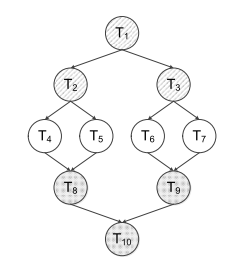
\includegraphics[width=0.5\textwidth]{./dados/figuras/mergesort}
    \fonte{\citeonline{pinto2013escalonamento}}
    \label{fig:figura-mergesort}
\end{figure}

A \autoref{fig:figura-mergesort} demonstra um grafo de dependência de tarefas de um algoritmo de mergesort, nesse exemplo, as tarefas \emph{T1},\emph{T2} e \emph{T3} dividem a entrada inicial, cada uma com metade do tamanho (\emph{n/2}).
Cada metade é uma nova tarefa, sendo que são elas são, \emph{T4}, \emph{T5}, \emph{T6} E \emph{T7}, essas tarefas são responsáveis por ordenar os dados.
Apos isso, as tarefas \emph{T8}, \emph{T9} e \emph{T10} fazem a combinação das partes separadas.

Nesse exemplo é possível notar as dependências de dados que existem entre as tarefas, pois as tarefas de combinação não podem ser executadas antes que as tarefas de divisão e ordenação tenham sido concluídas;

Aplicações baseadas no paradigma de paralelismo de tarefas podem explorar mais os recursos computacionais quando direcionadas a um ambiente de execução.
Após o desenvolvedor descrever as tarefas e as suas dependências, o ambiente é responsável pelo agendamento de tarefas, transferência de dados e gerenciamento das dependências \cite{pinto2017visual}.

Para executar essas atividades descritas acima, o sistema de execução infere características sobre o código da aplicação, como a quantidade de tarefas implementadas, unidade de processamento disponível (quantidade de núcleos de CPU e de dispositivos de GPUs), duração estimada da tarefa, localidade dos dados e largura de interconexão.
Apos isso, o tempo de execução pode usar heurísticas de agendamento apropriadas e executar otimizações para obter um melhor desempenho \cite{pinto2017visual}.

\subsection{StarPU}
StarPU é um sistema de tempo de execução que oferece suporte a arquiteturas multicore heterogêneas, oferecendo uma visão unificada dos recursos computacionais (CPUs e aceleradores ao mesmo tempo).
O ambiente implementa mecanismos para escalonar de forma eficiente as tarefas em uma arquitetura heterogênea \cite{augonnet2011scheduling}. 

Esta ferramenta tem como objetivo permitir que os programadores explorem o poder de computação das CPUs e GPUs disponíveis, ao mesmo tempo que em que os libera da necessidade de adaptar especialmente seus programas à máquina de destino e unidades de processamento.
StarPU é uma extensão para linguagens da família C (C Extensions), ela fornece uma API para descrever as tarefas e as suas dependências que podem existir em uma aplicação \cite{augonnet2011scheduling}.

\begin{citacao}
O modelo de execução do StarPU propõe uma abordagem de tarefas independente da arquitetura base.
São definidos codelets como uma abstração de uma tarefa que pode ser executada em um núcleo de uma CPU multicore ou submetido a um acelerador.
Cada codelet pode ter múltiplas implementações, uma para cada arquitetura em que o codelet pode ser executado.
Cada implementação utiliza as linguagens de programação ou bibliotecas específicas para a arquitetura alvo.
Um codelet contém uma descrição dos dados e o tipo de acesso (leitura, escrita ou ambos).
Codelets são lançados de forma assíncrona. Com isso o escalonador pode reordenar as tarefas para melhorar o desempenho respeitando as dependências entre elas.
Uma aplicação StarPU é descrita como um conjunto de codelets com suas dependências de dados. \cite[p.~26]{pinto2011ambientes}
\end{citacao}
\section{Transferência de Calor em Placas Metálicas}
% % REVISÃO DE LITERATURA--------------------------------------------------------

\chapter{REVISÃO DE LITERATURA}
\label{chap:fundamentacaoTeorica}

É uma boa prática iniciar cada novo capítulo com um breve texto introdutório (tipicamente, dois ou três parágrafos) que deve deixar claro o quê será discutido no capítulo, bem como a organização do capítulo.
Também servirá ao propósito de "amarrar"{} o conteúdo deste capítulo com o conteúdo do capítulo imediatamente anterior.
         % Revisão de Literatura
% % METODOLOGIA------------------------------------------------------------------

\chapter{METODOLOGIA}
\label{chap:metodologia}

Para conseguir explorar os ambientes de execução em arquiteturas heterogêneas será necessário desenvolver uma aplicação.
Essa aplicação que será desenvolvida será a de uma simulação de transferência de calor em uma placa metálica bidimensional,
utilizando a decomposição cartesiana.

Inicialmente, será feita uma pesquisa sobre arquiteturas heterogêneas e como funcionam os ambientes de execução para estas arquiteturas,
mais especificamente o ambiente StarPU.
Também serão estudados alguns trabalhos relacionados, que utilizam este ambiente e o paradigma de grafo de dependências de tarefas.

Posterior a isso, será realizado a implementação sequencial da simulação.
Este passo é interessante para entender como funciona a transferência de calor, utilizando a decomposição cartesiana e as dependências de
dados que existem na aplicação.

Apos a implementação sequencial, será necessário estudar e configurar o ambiente StarPU. Para a configuração do mesmo,
será estudado a documentação do ambiente e implementado alguns scripts do próprio tutorial.
O tutorial do StarPU é importante tanto para entender como funciona o ambiente de execução, como para configurar de forma correta o ambiente.

Em seguida, será realizado a implementação paralela da simulação de transferência de calor.
Para isto, será utilizado o paradigma de grafos de dependências de tarefas e executada no ambiente StarPU.

Por fim, será verificado qual é a melhor técnica de análise de desempenho para os dados obtidos nas execuções,
para então, ser concluído se aplicação paralela teve melhor desempenho, ou não, quando comparada com a aplicação sequencial.                   % Metodologia
% % RESULTADOS-------------------------------------------------------------------

\chapter{ANÁLISE E DISCUSSÃO DOS RESULTADOS}

Cada capítulo deve conter uma pequena introdução (tipicamente, um ou dois parágrafos) que deve deixar claro o objetivo e o que será discutido no capítulo, bem como a organização do capítulo.
                    % Resultados
% % ORIENTAÇÕES GERAIS------------------------------------------------------------


% SOBRE AS ILUSTRAÇÕES----------------------------------------------------------
\chapter{SOBRE AS ILUSTRAÇÕES}
\label{chap:apSobreIlust}

A seguir exemplifica-se como inserir ilustrações no corpo do trabalho. As ilustrações serão indexadas automaticamente em suas respectivas listas. A numeração sequencial de figuras, tabelas e equações também ocorre de modo automático.

Referências cruzadas são obtidas através dos comandos \verb|\label{}| e \verb|\ref{}|. Sendo assim, não é necessário por exemplo, saber que o número de certo capítulo é \ref{chap:fundamentacaoTeorica} para colocar o seu número no texto. Outra forma que pode ser utilizada é esta: \autoref{chap:fundamentacaoTeorica}, facilitando a inserção, remoção e manejo de elementos numerados no texto sem a necessidade de renumerar todos esses elementos.

% FIGURAS-----------------------------------------------------------------------
\chapter{FIGURAS}
\label{chap:figuras}

Exemplo de como inserir uma figura. A \autoref{fig:figura-exemplo1} aparece automaticamente na lista de figuras. Para saber mais sobre o uso de imagens no \LaTeX{} consulte literatura especializada \cite{Goossens2007}.

Os arquivos das figuras devem ser armazenados no diretório de "/dados".

\begin{figure}[!htb]
    \centering
    \caption{Exemplo de Figura}
    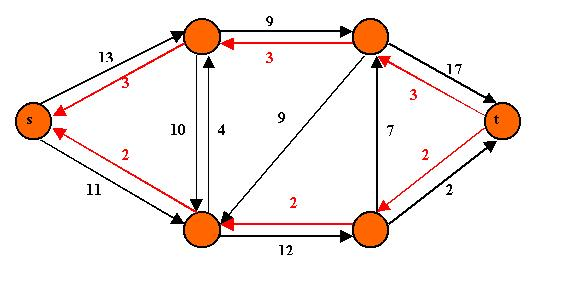
\includegraphics[width=0.5\textwidth]{./dados/figuras/figura1}
    \fonte{\citeonline{IRL2014}}
    \label{fig:figura-exemplo1}
\end{figure}

% QUADROS E TABELAS---------------------------------------------------------------
\chapter{QUADROS E TABELAS}
\label{chap:tabelas}

Exemplo de como inserir o \autoref{qua:quadro-exemplo1} e a \autoref{tab:tabela-exemplo1}. Ambos aparecem automaticamente nas suas respectivas listas. Para saber mais informações sobre a construção de tabelas no \LaTeX{} consulte literatura especializada \cite{Mittelbach2004}.

Ambos os elementos (Quadros e Tabelas) devem ser criados em arquivos separados para facilitar manutenção e armazenados no diretório de "/dados".

\begin{quadro}[!htb]
    \centering
    \caption{Exemplo de Quadro.\label{qua:quadro-exemplo1}}
    \begin{tabular}{|p{7cm}|p{7cm}|}
        \hline
        \textbf{BD Relacionais} & \textbf{BD Orientados a Objetos} \\
        \hline
        Os dados são passivos, ou seja, certas operações limitadas podem ser automaticamente acionadas quando os dados são usados. Os dados são ativos, ou seja, as solicitações fazem com que os objetos executem seus métodos. & Os processos que usam dados mudam constantemente. \\
        \hline
    \end{tabular}
    \fonte{\citeonline{Barbosa2004}}
\end{quadro}


A diferença entre quadro e tabela está no fato que um quadro é formado por linhas horizontais e verticais. Deve ser utilizado quando o conteúdo é majoritariamente não-numérico. O número do quadro e o título vem acima do quadro, e a fonte, deve vir abaixo. E Uma tabela é formada apenas por linhas verticais. Deve ser utilizada quando o conteúdo é majoritariamente numérico. O número da tabela e o título vem acima da tabela, e a fonte, deve vir abaixo, tal como no quadro.

\begin{table}[!htb]
    \centering
    \caption[Resultado dos testes]{Resultado dos testes.
    \label{tab:tabela-exemplo1}}
    \begin{tabular}{rrrrr}
        \toprule
            & Valores 1 & Valores 2 & Valores 3 & Valores 4 \\
        \midrule
            Caso 1 & 0,86 & 0,77 & 0,81 & 163 \\
            Caso 2 & 0,19 & 0,74 & 0,25 & 180 \\
            Caso 3 & 1,00 & 1,00 & 1,00 & 170 \\
        \bottomrule
    \end{tabular}
    \fonte{\citeonline{Barbosa2004}}
\end{table}


% EQUAÇÕES-----------------------------------------------------------------------
\chapter{EQUAÇÕES}
\label{chap:equacoes}

Exemplo de como inserir a \autoref{eq:equacao-exemplo1} e a Eq. \ref{eq:equacao-exemplo2} no corpo do texto \footnote{Deve-se atentar ao fato de a formatação das equações ficar muito boa esteticamente.}. Observe que foram utilizadas duas formas distintas para referenciar as equações.

\begin{equation}
    X(s) = \int\limits_{t = -\infty}^{\infty} x(t) \, \text{e}^{-st} \, dt
    \label{eq:equacao-exemplo1}
\end{equation}

\begin{equation}
    F(u, v) = \sum_{m = 0}^{M - 1} \sum_{n = 0}^{N - 1} f(m, n) \exp \left[ -j 2 \pi \left( \frac{u m}{M} + \frac{v n}{N} \right) \right]
    \label{eq:equacao-exemplo2}
\end{equation}

% ALGORITMOS-----------------------------------------------------------------------
\chapter{ALGORITMOS}
\label{chap:algoritmos}

Exemplo de como inserir um algoritmo. Para inserção de algoritmos utiliza-se o pacote {\ttfamily algorithm2e} que já está devidamente configurado dentro do template.

Os algoritmos devem ser criados em arquivos separados para facilitar manutenção e armazenados no diretório de "/dados".\\
\\

\begin{algorithm}
    \caption{Exemplo de Algoritmo}
    \KwIn{o número $n$ de vértices a remover, grafo original $G(V, E)$}
    \KwOut{grafo reduzido $G'(V,E)$}
    $removidos \leftarrow 0$ \\
    \While {removidos $<$ n } {
        $v \leftarrow$ Random$(1, ..., k) \in V$ \\
            \For {$u \in adjacentes(v)$} {
                remove aresta (u, v)\\
                $removidos \leftarrow removidos + 1$\\
            }
            \If {há  componentes desconectados} {
                remove os componentes desconectados\\
            }
        }
\end{algorithm}


% SOBRE AS LISTAS--------------------------------------------------------------------
\chapter{SOBRE AS LISTAS}
\label{chap:apSobreLista}

Para construir listas de "\textit{bullets}"{} ou listas enumeradas, inclusive listas aninhadas, é utilizado o pacote \verb|paralist|.

Exemplo de duas listas não numeradas aninhadas, utilizando o comando \verb|\itemize|. Observe a indentação, bem como a mudança automática do tipo de "\textit{bullet}"{} nas listas aninhadas.

\begin{itemize}
    \item item não numerado 1
    \item item não numerado 2
    \begin{itemize}
        \item subitem não numerado 1
        \item subitem não numerado 2
        \item subitem não numerado 3
    \end{itemize}
    \item item não numerado 3
\end{itemize}

Exemplo de duas listas numeradas aninhadas, utilizando o comando \verb|\enumerate|. Observe a numeração progressiva e indentação das listas aninhadas.

\begin{enumerate}
    \item item numerado 1
    \item item numerado 2
    \begin{enumerate}
        \item subitem numerado 1
        \item subitem numerado 2
        \item subitem numerado 3
    \end{enumerate}
    \item item numerado 3
\end{enumerate}

% SOBRE AS CITAÇÕES E CHAMADAS DE REFERÊNCAS----------------------------------------------
\chapter{SOBRE AS CITAÇÕES E CHAMADAS DE REFERÊNCAS}
\label{chap:apSobreCita}

Citações são trechos de texto ou informações obtidas de materiais consultadss quando da elaboração do trabalho. São utilizadas no texto com o propósito de esclarecer, completar e embasar as ideias do autor. Todas as publicações consultadas e utilizadas (por meio de citações) devem ser listadas, obrigatoriamente, nas referências bibliográficas, para preservar os direitos autorais. São classificadas em citações indiretas e diretas.

% CITAÇÕES INDIRETAS-----------------------------------------------------------------------
\chapter{CITAÇÕES INDIRETAS}
\label{chap:citacoesLivres}

É a transcrição, com suas próprias palavras, das idéias de um autor, mantendo-se o sentido original. A citação indireta é a maneira que o pesquisador tem de ler, compreender e gerar conhecimento a partir do conhecimento de outros autores. Quanto à chamada da referência, ela pode ser feita de duas maneiras distintas, conforme o nome do(s) autor(es) façam parte do seu texto ou não. Exemplo de chamada fazendo parte do texto:\\
\\Enquanto \citeonline{Maturana2003} defendem uma epistemologia baseada na biologia. Para os autores, é necessário rever \ldots.\\

A chamada de referência foi feita com o comando \verb|\citeonline{chave}|, que produzirá a formatação correta.

A segunda forma de fazer uma chamada de referência deve ser utilizada quando se quer evitar uma interrupção na sequência do texto, o que poderia, eventualmente, prejudicar a leitura. Assim, a citação é feita e imediatamente após a obra referenciada deve ser colocada entre parênteses. Porém, neste caso específico, o nome do autor deve vir em caixa alta, seguido do ano da publicação. Exemplo de chamada não fazendo parte do texto:\\
\\Há defensores da epistemologia baseada na biologia que argumentam em favor da necessidade de \ldots \cite{Maturana2003}.\\

Nesse caso a chamada de referência deve ser feita com o comando \verb|\cite{chave}|, que produzirá a formatação correta.

% CITAÇÕES DIRETAS-----------------------------------------------------------------------
\chapter{CITAÇÕES DIRETAS}
\label{chap:citacoesLiterais}

É a transcrição ou cópia de um parágrafo, de uma frase, de parte dela ou de uma expressão, usando exatamente as mesmas palavras adotadas pelo autor do trabalho consultado.

Quanto à chamada da referência, ela pode ser feita de qualquer das duas maneiras já mencionadas nas citações indiretas, conforme o nome do(s) autor(es) façam parte do texto ou não. Há duas maneiras distintas de se fazer uma citação direta, conforme o trecho citado seja longo ou curto.

Quando o trecho citado é longo (4 ou mais linhas) deve-se usar um parágrafo específico para a citação, na forma de um texto recuado (4 cm da margem esquerda), com tamanho de letra menor e espaçamento entrelinhas simples. Exemplo de citação longa:
\\\begin{citacao}
    Desse modo, opera-se uma ruptura decisiva entre a reflexividade filosófica, isto é a possibilidade do sujeito de pensar e de refletir, e a objetividade científica. Encontramo-nos num ponto em que o conhecimento científico está sem consciência. Sem consciência moral, sem consciência reflexiva e também subjetiva. Cada vez mais o desenvolvimento extraordinário do conhecimento científico vai tornar menos praticável a própria possibilidade de reflexão do sujeito sobre a sua pesquisa \cite[p.~28]{Silva2000}.
\end{citacao}

Para fazer a citação longa deve-se utilizar os seguintes comandos:
\begin{verbatim}
\begin{citacao}
<texto da citacao>
\end{citacao}
\end{verbatim}

No exemplo acima, para a chamada da referência o comando \verb|\cite[p.~28]{Silva2000}| foi utilizado, visto que os nomes dos autores não são parte do trecho citado. É necessário também indicar o número da página da obra citada que contém o trecho citado.

Quando o trecho citado é curto (3 ou menos linhas) ele deve inserido diretamente no texto entre aspas. Exemplos de citação curta:\\
\\A epistemologia baseada na biologia parte do princípio de que "assumo que não posso fazer referência a entidades independentes de mim para construir meu explicar" \cite[p.~35]{Maturana2003}.\\
\\A epistemologia baseada na biologia de \citeonline[p.~35]{Maturana2003} parte do princípio de que "assumo que não posso fazer referência a entidades independentes de mim para construir meu explicar".

% DETALHES SOBRE AS CHAMADAS DE REFERÊNCIAS---------------------------------------------------------
\chapter{DETALHES SOBRE AS CHAMADAS DE REFERÊNCIAS}
\label{chap:referUtilizadas}

Outros exemplos de comandos para as chamadas de referências e o resultado produzido por estes:\\
\\\citeonline{Maturana2003} \ \ \  \verb|\citeonline{Maturana2003}|\\
\citeonline{Barbosa2004} \ \ \   \verb|\citeonline{Barbosa2004}|\\
\cite[p.~28]{Silva2000} \ \ \  \verb|\cite[p.~28]{Silva2000}|\\
\citeonline[p.~33]{Silva2000} \ \ \   \verb|\citeonline[p.~33]{v}|\\
\cite[p.~35]{Maturana2003} \ \ \   \verb|\cite[p.~35]{Maturana2003}|\\
\citeonline[p.~35]{Maturana2003} \ \ \   \verb|\citeonline[p.~35]{Maturana2003}|\\
\cite{Barbosa2004,Maturana2003} \ \ \   \verb|\cite{Barbosa2004,Maturana2003}|\\

% SOBRE AS REFERÊNCIAS BIBLIOGRÁFICAS-------------------------------------------------------
\chapter{SOBRE AS REFERÊNCIAS BIBLIOGRÁFICAS}
\label{chap:apSobreRefer}

A bibliografia é feita no padrão \textsc{Bib}\TeX{}. As referências são colocadas em um arquivo separado. Neste template as referências são armazenadas no arquivo "base-referencias.bib".

Existem diversas categorias documentos e materiais componentes da bibliografia. A classe abn\TeX{} define as seguintes categorias (entradas):

\begin{verbatim}
@book
@inbook
@article
@phdthesis
@mastersthesis
@monography
@techreport
@manual
@proceedings
@inproceedings
@journalpart
@booklet
@patent
@unpublished
@misc
\end{verbatim}

Cada categoria (entrada) é formatada pelo pacote \citeonline{abnTeX22014d} de uma forma específica. Algumas entradas foram introduzidas especificamente para atender à norma \citeonline{NBR6023:2002}, são elas: \verb|@monography|, \verb|@journalpart|,\verb|@patent|. As demais entradas são padrão \textsc{Bib}\TeX{}. Para maiores detalhes, refira-se a \citeonline{abnTeX22014d}, \citeonline{abnTeX22014b}, \citeonline{abnTeX22014c}.

% NOTAS DE RODAPÉ--------------------------------------------------------------------------
\chapter{NOTAS DE RODAPÉ}
\label{chap:notasRodape}

As notas de rodapé pode ser classificadas em duas categorias: notas explicativas\footnote{é o tipo mais comum de notas que destacam, explicam e/ou complementam o que foi dito no corpo do texto, como esta nota de rodapé, por exemplo.} e notas de referências. A notas de referências, como o próprio nome ja indica, são utilizadas para colocar referências e/ou chamadas de referências sob certas condições.
                   % Capítulo com Orientações de uso do Template
% % CONCLUSÃO--------------------------------------------------------------------

\chapter{CONCLUSÃO}
\label{chap:conclusao}

Parte final do texto, na qual se apresentam as conclusões do trabalho acadêmico. É importante fazer uma análise crítica do trabalho, destacando os principais resultados e as contribuições do trabalho para a área de pesquisa.

\section{TRABALHOS FUTUROS}
\label{sec:trabalhosFuturos}

Também deve indicar, se possível e/ou conveniente, como o trabalho pode ser estendido ou aprimorado.

\section{CONSIDERAÇÕES FINAIS}
\label{sec:consideracoesFinais}

Encerramento do trabalho acadêmico.
                 			   % Conclusão

\postextual
% INSERE ELEMENTOS PÓS-TEXTUAIS
% REFERÊNCIAS------------------------------------------------------------------

% Carrega o arquivo "exemplo-referencias.bib" e extrai automaticamente as referências citadas
{\renewcommand{\contentsname}{MAC}}
\bibliography{./exemplo-referencias}
\bibliographystyle{abntex2-alf} % Define o estilo ABNT para formatar a lista de referências
% OBSERVAÇÕES------------------------------------------------------------------
% Este arquivo não precisa ser alterado.           			   % Referências
% % APÊNDICES--------------------------------------------------------------------

\begin{apendicesenv}
\partapendices

% Primeiro apêndice------------------------------------------------------------
\chapter{Nome do apêndice} % Edite para alterar o título deste apêndice
\label{chap:apendiceA}

Lembre-se que a diferença entre apêndice e anexo diz respeito à autoria do texto e/ou material ali colocado.

Caso o material ou texto suplementar ou complementar seja de sua autoria, então ele deverá ser colocado como um apêndice. Porém, caso a autoria seja de terceiros, então o material ou texto deverá ser colocado como anexo.

Caso seja conveniente, podem ser criados outros apêndices para o seu trabalho acadêmico. Basta recortar e colar este trecho neste mesmo documento. Lembre-se de alterar o "label"{} do apêndice.

Não é aconselhável colocar tudo que é complementar em um único apêndice. Organize os apêndices de modo que, em cada um deles, haja um único tipo de conteúdo. Isso facilita a leitura e compreensão para o leitor do trabalho.

% Novo apêndice----------------------------------------------------------------
\chapter{Nome do outro apêndice}
\label{chap:apendiceB}

conteúdo do novo apêndice

\end{apendicesenv}
             			   % Apêndices
% % ANEXO------------------------------------------------------------------------

\begin{anexosenv}
\partanexos

% Primeiro anexo---------------------------------------------------------------
\chapter{Nome do anexo}     % edite para alterar o título deste anexo
\label{chap:anexoA}

Lembre-se que a diferença entre apêndice e anexo diz respeito à autoria do texto e/ou material ali colocado.

Caso o material ou texto suplementar ou complementar seja de sua autoria, então ele deverá ser colocado como um apêndice. Porém, caso a autoria seja de terceiros, então o material ou texto deverá ser colocado como anexo.

Caso seja conveniente, podem ser criados outros anexos para o seu trabalho acadêmico. Basta recortar e colar este trecho neste mesmo documento. Lembre-se de alterar o "label"{} do anexo.

Organize seus anexos de modo a que, em cada um deles, haja um único tipo de conteúdo. Isso facilita a leitura e compreensão para o leitor do trabalho. É para ele que você escreve.

% Novo anexo-------------------------------------------------------------------
\chapter{Nome do outro anexo}
\label{chap:anexoB}

conteúdo do outro anexo

\end{anexosenv}
               			   % Anexos

\end{document}
